% Este trabalho está licenciado sob a Licença Atribuição-CompartilhaIgual 4.0 Internacional Creative Commons. Para visualizar uma cópia desta licença, visite http://creativecommons.org/licenses/by-sa/4.0/deed.pt_BR ou mande uma carta para Creative Commons, PO Box 1866, Mountain View, CA 94042, USA.

\chapter{Funções}\label{cap_fun}
\thispagestyle{fancy}

Uma \hl{\emph{função} (ou método) é um \emph{subprograma} (ou subalgoritmo)}, um bloco de programação para o processamento de uma tarefa e que pode ser chamado à execução, sempre que necessário, pelo programa a que pertence.

\section{Funções Predefinidas e Módulos}\label{cap_fun_sec_buildin}

\subsection{Funções Predefinidas}

Como o nome indica, \hl{\emph{funções predefinidas} são aquelas disponíveis por padrão na linguagem de programação}, i.e. sem a necessidade de serem explicitamente definidas no código. As \hl{funções predefinidas do {\python}} podem ser consultadas em
\begin{center}
  \url{https://docs.python.org/3/library/functions.html}
\end{center}

Nós já vinhamos utilizando várias dessas funções.

\subsubsection{Entrada e Saída de Dados}

Na entrada e saída de dados, utilizamos
\begin{itemize}
\item \hl{{\lstinline+input()+}}

  Essa função lê uma linha digitada no \textit{prompt}, converte-a em uma \textit{string} e a retorna. Admite como entrada uma \textit{string} que é impressa no \textit{prompt} antes da leitura.

\item \hl{{\lstinline+print()+}}

  Essa função recebe um objeto e o imprime em formato texto, por padrão, no \textit{prompt} de saída.

\begin{lstlisting}
>>> s = input('Olá, qual o seu nome? ')
Olá, qual o seu nome? Fulane
>>> print(f'Bem vinde, {s}!')
Bem vinde, Fulane!
\end{lstlisting}
\end{itemize}

\subsubsection{Construtores de Dados}

Temos as funções que constroem objetos de classes de números:
\begin{itemize}

\item \hl{{\lstinline+bool()+}}

  Recebe um objeto e retorna outro da classe \lstinline+bool+.

\begin{lstlisting}
>>> bool(0)
False
>>> bool(1)
True
>>> bool('')
False
>>> bool('0')
True
\end{lstlisting}
  
\item \hl{{\lstinline+int()+}}

  Recebe um número ou \textit{string} \lstinline+x+ e retorna um objeto da classe \lstinline+int+.

\begin{lstlisting}
>>> int(-2.1)
-2
>>> int(3.9)
3
>>> int(5.5)
5
>>> int('51')
51
\end{lstlisting}

\item \hl{{\lstinline+float()+}}

  Recebe um número ou \textit{string} \lstinline+x+ e retorna um objeto da classe \lstinline+float+.

\begin{lstlisting}
>>> float(1)
1.0
>>> float('-2.7')
-2.7
\end{lstlisting}

\item \hl{{\lstinline+complex()+}}

  Recebe as partes real e imaginária de um número complexo ou uma \textit{string} e retorna um objeto da classe \lstinline+complex+.

\begin{lstlisting}
>>> complex(2,-3)
(2-3j)
>>> complex('-7+5j')
(-7+5j)
\end{lstlisting}
\end{itemize}

Para a construção de objetos de classes de coleção de dados, temos:
\begin{itemize}
\item \hl{{\lstinline+dict()+}}

  Recebe um mapeamento ou um iterável e retorna um objeto da classe \lstinline+dict+.

\item \hl{{\lstinline+list()+}}

  Recebe um iterável e retorna um objeto da classe \lstinline+list+.

\item \hl{{\lstinline+set()+}}

  Recebe um iterável e retorna um objeto da classe \lstinline+set+.

\item \hl{{\lstinline+str()+}}

  Recebe um objeto e retorna um outro da classe \lstinline+str+

\item \hl{{\lstinline+tuple+}}

  Recebe um iterável e retorna um objeto da classe \lstinline+tuple+.
\end{itemize}

Alguns construtores de iteráveis especiais são:
\begin{itemize}
\item \hl{{\lstinline+range()+}}

  Recebe até três inteiros \lstinline+start+, \lstinline+stop+, \lstinline+step+ e retorna um objeto iterável com início em \lstinline+start+ (incluído) e término em \lstinline+stop+ (excluído).

\begin{lstlisting}
>>> list(range(5))
[0, 1, 2, 3, 4]
>>> tuple(range(-10,1,2))
(-10, -8, -6, -4, -2, 0)
\end{lstlisting}

\item \hl{{\lstinline+enumerator()+}}

  Recebe um iterável e retorna um objeto \lstinline+enumerate+, um iterável de tuples que enumera os objetos do iterável de entrada.

\begin{lstlisting}
>>> cores = ['amarelo', 'azul', 'vermelho', ]
>>> list(enumerate(cores))
[(0, 'amarelo'), (1, 'azul'), (2, 'vermelho')]
\end{lstlisting}
\end{itemize}

\subsection{Módulos}

\hl{Módulos são bibliotecas computacionais}, i.e. um arquivo contendo funções (e/ou constantes) que podem ser incorporadas e usadas em outros programas. Existem vários módulos disponíveis na linguagem {\python}, para citar alguns:
\begin{itemize}
\item \hl{{\lstinline+math+}} : módulo de matemática elementar.
\item \hl{{\lstinline+random+}} : módulo de números randômicos.
\item \hl{{\lstinline+numpy+}} : módulo de computação matricial.
\item \hl{{\lstinline+matplotlib+}} : módulo de vizualização gráfica.
\item \hl{{\lstinline+sympy+}} : módulo de matemática simbólica.
\item \hl{{\lstinline+torch+}} : módulo de aprendizagem de máquina.
\end{itemize}

Nesta seção vamos apenas introduzir o módulo \lstinline+math+. Mais a frente, também fazemos uma introdução aos módulos \lstinline+numpy+ e \lstinline+matplotlib+.

\subsubsection{Módulo \lstinline+math+}

\hl{O módulo {\lstinline+math+} fornece acesso a constantes e funções matemáticas elementares para números reais}. Para \hl{\emph{importar o módulo}} em nosso código, podemos usar a instrução \hl{{\lstinline+import+}}. Por exemplo,
\begin{lstlisting}
>>> import math
>>> help(math)
\end{lstlisting}
Então, para usar algum recurso do módulo usamos \hl{{\lstinline+math.+}} seguido do nome do recurso que queremos. Por exemplo,
\begin{lstlisting}
>>> math.e
2.718281828459045
\end{lstlisting}
retorna o número de Euler{\euler} em ponto flutuante.

Alternativamente, podemos importar o módulo com o nome que quisermos. Por padrão, usa-se
\begin{lstlisting}
>>> import math as m
>>> m.pi
3.141592653589793
\end{lstlisting}
Ainda, pode-se importar apenas um ou mais recursos específicos, por exemplo\footnote{\faIcon[regular]{grin-wink}}
\begin{lstlisting}
>>> from math import pi, sin, cos
>>> sin(pi)**2 + cos(pi) == 1
False
\end{lstlisting}

\begin{ex}
  Considere um polinômio de segundo grau da forma
  \begin{equation}
    p(x) = ax^2 + bx + c.
  \end{equation}
  O seguinte código, computa as raízes de $p$ para valores dos coeficientes fornecidos por usuária(o).

\begin{lstlisting}
import math as m

# entrada de dados
a = float(input('Digite o valor de a:\n'))
b = float(input('Digite o valor de b:\n'))
c = float(input('Digite o valor de c:\n'))

# discriminante
delta = b**2 - 4*a*c

# raízes
# raízes distintas
if (delta > 0):
    x1 = (-b + m.sqrt(delta))/(2*a)
    x2 = (-b - m.sqrt(delta))/(2*a)
# raiz dupla
elif (delta == 0):
    x1 = -b/(2*a)
    x2 = x1
# raízes complexas
else:
    real = -b/(2*a)
    img = m.sqrt(-delta)/(2*a)
    x1 = complex(real, img)
    x2 = x1.conjugate()

print(f'x1 = {x1}')
print(f'x2 = {x2}')
\end{lstlisting}
\end{ex}

\subsection{Exercícios}

\begin{exer}
  Desenvolva um código que computa e imprime a hipotenusa $h$ de um triângulo retângulo com catetos $a$ e $b$ fornecidos por usuária(o).
\end{exer}
\begin{resp}
  Dica: use \lstinline+h = math.sqrt(a**2 + b**2)+.
\end{resp}

\begin{exer}
  Um triângulo de lados $a$, $b$ e $c$, existe se
  \begin{equation}
    |b-c| < a < b + c.
  \end{equation}
  Desenvolva um código que verifica e informa a existência de um triângulo de lados fornecidos por usuária(o).
\end{exer}
\begin{resp}
  Dica: verifique a condição \lstinline+(m.fabs(b-c) < a) and (a < b+c)+
\end{resp}

\begin{exer}
  Considere um triangulo com as seguintes medidas
  \begin{figure}[H]
    \centering
    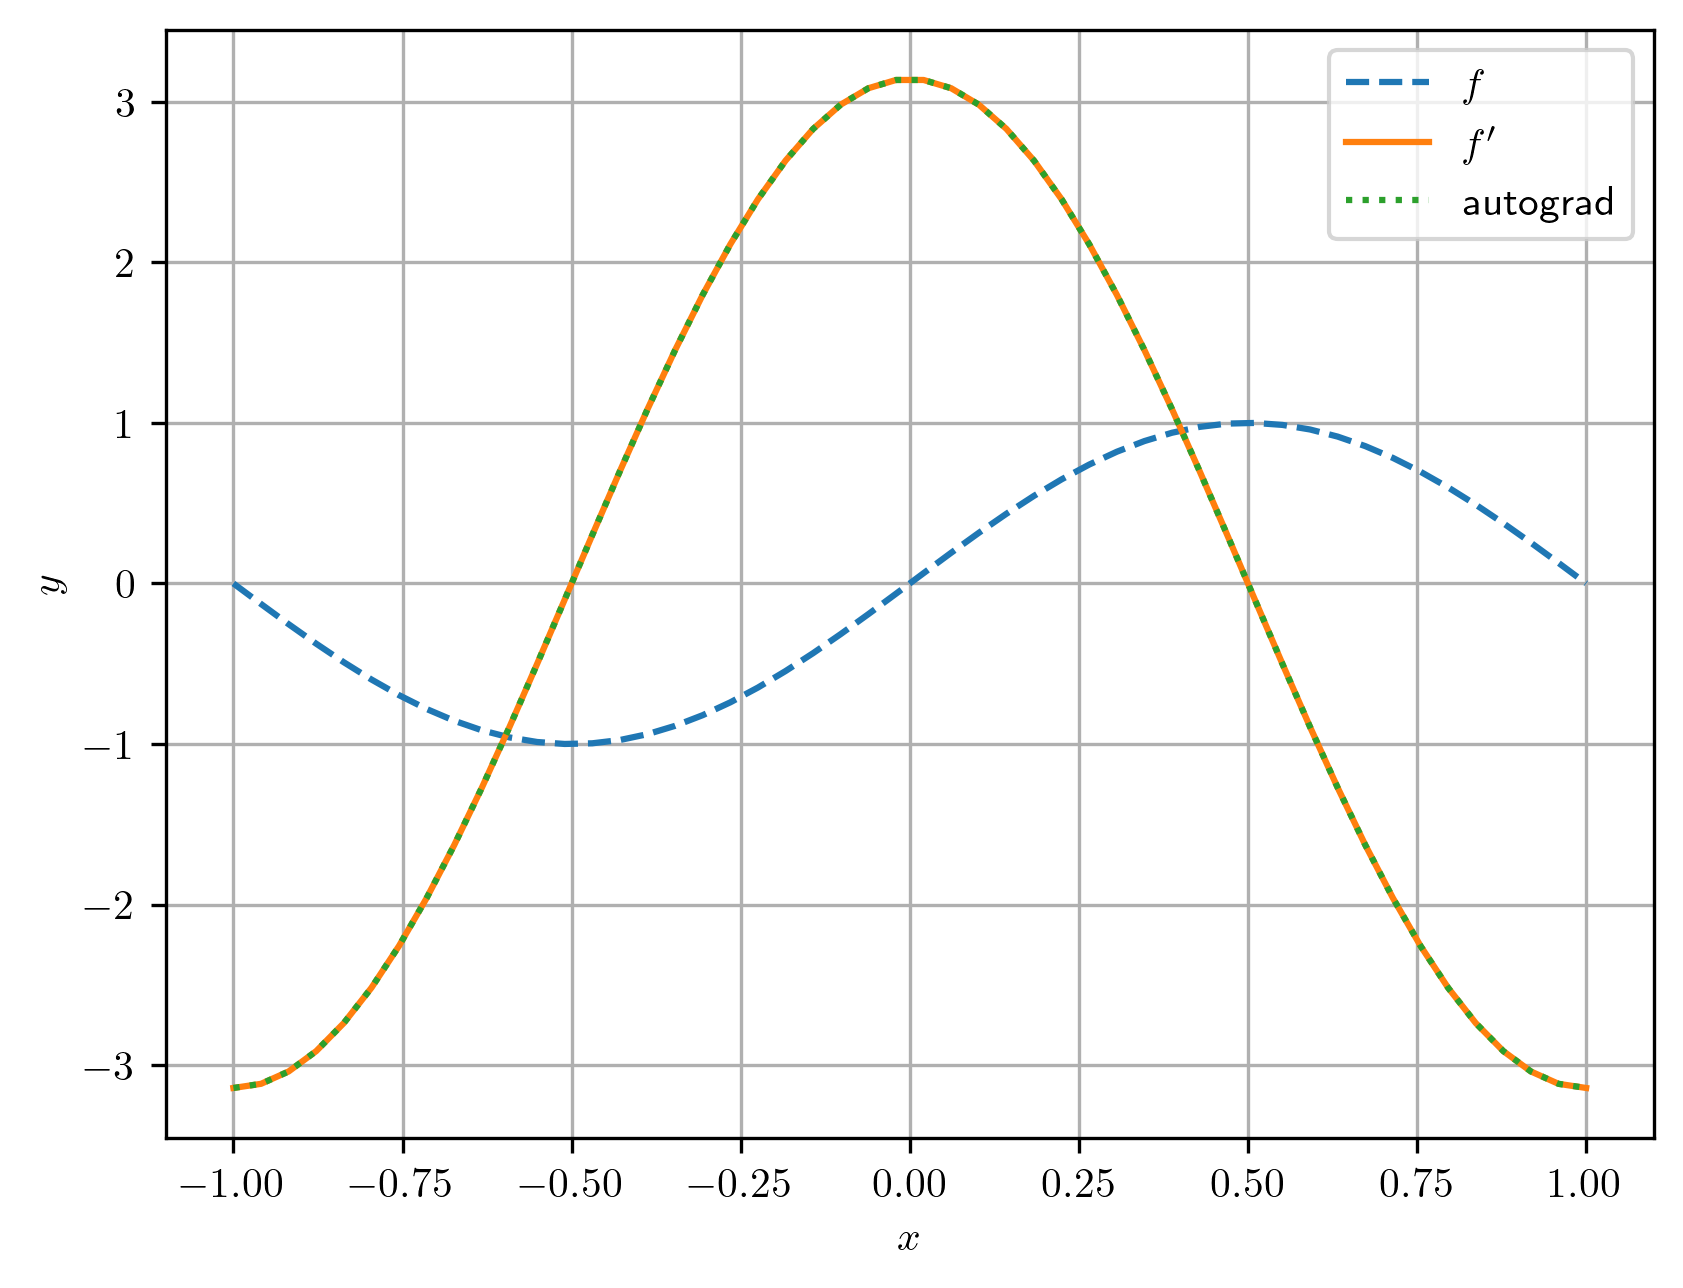
\includegraphics[width=0.4\textwidth]{./cap_fun/dados/fig_leiDosCossenos/fig}
  \end{figure}
  Desenvolva um código que computa e imprime o valor da área de um triangulo de lados $a$, $b$ e $c$ fornecidos por usuária(o).
\end{exer}
\begin{resp}
  Dica: use a \href{https://pt.wikipedia.org/wiki/Lei_dos_cossenos}{lei dos cossenos} e relações fundamentais de triangulo retângulo para obter o valor da altura $h$. 
\end{resp}

\begin{exer}
  Desenvolva um código em que a(o) usuária forneça um ângulo $\theta$ em graus e seja computado e impresso os $\sen(\theta)$ e $\cos(\theta)$.
\end{exer}
\begin{resp}
  Dica: consulte as funções \lstinline+math.sin+, \lstinline+math.cos+.
\end{resp}

\begin{exer}
  Desenvolva um jogo em que a(o) usuária(o) tenha três tentativas para adivinhar um número inteiro entre $0$ a $51$ (incluídos). 
\end{exer}
\begin{resp}
  Dica: O módulo \lstinline+random+ fornece a função \href{https://docs.python.org/3/library/random.html?highlight=random#random.randint}{\lstinline+random.randint(a, b)+} que retorna um inteiro $a \leq x \leq b$.
\end{resp}

\section{Definindo Funções}\label{cap_fun_sec_def}

Em {\python}, criamos ou \hl{definimos uma função com a instrução {\lstinline+def+}}, com a seguinte sintaxe
\begin{lstlisting}
def foo(x):
   bloco
\end{lstlisting}
Aqui, \lstinline+foo+ é o nome da função, \lstinline+x+ é o parâmetro (variável) de entrada e \lstinline+bloco+ é o bloco de programação que a função executa ao ser chamada. Uma função pode ter mais parâmetros ou não ter parâmetro de entrada.

\begin{ex}\label{cap_fun_sec_def:ex:areaCirc}
  O seguinte código, define a função \lstinline+areaCirc+ que computa e imprime a área de uma circunferência de raio $r$.
\begin{lstlisting}
import math as m

def areaCirc(r):
    area = m.pi * r**2
    print(f'área = {area}')
\end{lstlisting}
  Uma vez definida, a função pode ser chamada em qualquer parte do código. Por exemplo, vamos continuar o código de forma que a(o) usuária(o) informe os raios de duas circunferências e o código compute e imprima o valor das áreas de cada circunferência.
\begin{lstlisting}
import math as m

# def fun
def areaCirc(r):
    area = m.pi * r**2
    print(f'área = {area}')
    
# entrada de dados
raio1 = float(input('Digite o raio da 1. circ.:\n'))
raio2 = float(input('Digite o raio da 2. circ.:\n'))

print(f'Circunferência de raio = {raio1}')
areaCirc(raio1)

print(f'Circunferência de raio = {raio2}')
areaCirc(raio2)
\end{lstlisting}
\end{ex}

\begin{obs}\normalfont{(\hl{{\lstinline+docstring+}}.)}
  {\python} recomenda a utilização do sistema de documentação \lstinline+docstring+. Na definição de funções, um pequeno comentário sobre sua funcionalidade, seguido da descrição sobre seus parâmetros podem ser feito usando \lstinline+'''+, logo abaixo da instrução \lstinline+def+. Por exemplo,
\begin{lstlisting}
import math as m

# def fun
def areaCirc(r):
    '''
    Computa e imprime a área de uma
    circunferência.

    Entrada
    -------
    r : float
    Raio da circunferência.
    '''
    area = m.pi * r**2
    print(f'área = {area}')
\end{lstlisting}
  Com isso, podemos usar a função \lstinline+help+ para obter a documentação da função \lstinline+areaCirc+.
\begin{lstlisting}
>>> help(areaCirc)
\end{lstlisting}
  Verifique!
\end{obs}

Uma função pode ser definida sem parâmetro de entrada.

\begin{ex}
  O seguinte código, implementa uma função que imprime um número randômico par entre $0$ e $100$ (incluídos).
\begin{lstlisting}
import random

def randPar100():
    '''
    Imprime um número randômico
    par entre 0 e 100 (incluídos).
    '''
    n = random.randint(0, 99)
    if (n % 2 == 0):
        print(n)
    else:
        print(n+1)
\end{lstlisting}
  Para chamá-la, usamos
\begin{lstlisting}
>>> randPar100()
\end{lstlisting}
  Verifique!
\end{ex}

\subsection{Funções com Saída de Dados}

Além de parâmetros de entrada, \hl{uma função pode ter saída de dados}, i.e. pode retornar dados para o programa. Para isso, usamos a instrução \lstinline+return+ que interrompe a execução da função e retorna ao programa principal. Quando o \lstinline+return+ é seguido de um objeto, a função tem como saída o valor desse objeto.

\begin{ex}
  Vamos atualizar a versão de nosso código do Exemplo \ref{cap_fun_sec_def:ex:areaCirc}. Aqui, em vez de imprimir, a função \lstinline+areaCirc(r)+ tem como saída o valor computado da área da circunferência de raio \lstinline+r+
\begin{lstlisting}
import math as m

# def fun
def areaCirc(r):
    area = m.pi * r**2
    return area
    
# entrada de dados
raio1 = float(input('Digite o raio da 1. circ.:\n'))
raio2 = float(input('Digite o raio da 2. circ.:\n'))

print(f'Circunferência de raio = {raio1}')
area1 = areaCirc(raio1)
print(f'\tárea = {area1}')

print(f'Circunferência de raio = {raio2}')
area2 = areaCirc(raio2)
print(f'\tárea = {area2}')
\end{lstlisting}
\end{ex}

Funções podem retornar objetos de qualquer classe de dados. Quando queremos retornar mais de um objeto por vez, usualmente usamos um \lstinline+tuple+ como variável de saída.

\begin{ex}
  O seguinte código, cria uma função para a computação das raízes de um polinômio de grau 2
  \begin{equation}
    p(x) = ax^2 + bx + c.
  \end{equation}
\begin{lstlisting}[caption=raizes\_v1.py, label=cap_progest_sec_def:cod:raizes_v1]
import math as m

def raizes(a, b, c):
    '''
    Computa as raízes de
    p(x) = ax^2 + bx + c

    Entrada
    -------
    a : float
    Coeficiente do termo quadrático.
    Atenção! Deve ser diferente de zero.

    b : float 
    Coeficiente do termo linear.

    c: float
    Coeficiente do termo constante.

    Saída
    -----
    x1 : float
    Uma raíz do polinômio.

    x2 : float
    Outra raíz do polinômio.
    Atenção! No caso de raiz dupla,
    x1 == x2.
    '''

    # auxiliares
    _2a = 2*a
    _b2a = -b/_2a

    # discriminante
    delta = b**2 - 4*a*c

    # raízes
    if (delta > 0):
        x1 = _b2a + m.sqrt(delta)/_2a
        x2 = _b2a - m.sqrt(delta)/_2a
        return x1, x2
    elif (delta < 0):
        img = m.sqrt(-delta)/_2a
        x1 = _b2a + img*1j
        return x1, x1.conjugate()
    else:
        return _b2a, _b2a
\end{lstlisting}
  Verifique!
\end{ex}

\subsection{Capturando Exceções}

\hl{Exceções são classes de erros encontrados durante a execução de um código}. Ao encontrar uma exceção, a execução do código {\python} é imediatamente interrompida e uma mensagem é impressa indicando a classe do erro e a linha do código em ocorreu. Por exemplo, ao chamarmos \lstinline+raizes(0, 1, 2)+ definida no Código \ref{cap_progest_sec_def:cod:raizes_v1}, obtemos uma exceção da classe \lstinline+ZeroDivisionError+.
\begin{lstlisting}
>>> raizes(0,1,2)
Traceback (most recent call last):
  File "<stdin>", line 1, in <module>
  File "/home/pkonzen/GitHub/notas/src/AlgoritmosProgramacaoI/cap_fun/dados/aux.py", line 33, in raizes
    _b2a = -b/_2a
ZeroDivisionError: division by zero
\end{lstlisting}

Podemos controlar as exceções com a instrução \lstinline+try-except+. Sua sintaxe é
\begin{lstlisting}
try:
    comando1
except:
    comando2
\end{lstlisting}
Ou seja, o código tenta executar o \lstinline+comando1+, caso ele gere uma exceção, o \lstinline+comando2+ é executado. A lista de exceções predefinidas na linguagem pode ser consultada em
\begin{center}
  \url{https://docs.python.org/3/library/exceptions.html}
\end{center}

\begin{ex}
  No Código \ref{cap_progest_sec_def:cod:raizes_v1}, podemos evitar e avisar a(o) usuária(o) da divisão por zero no caso de $a=0$.
\begin{lstlisting}[caption=raizes\_v2.py]
import math as m

def raizes(a, b, c):
    '''
    Computa as raízes de
    p(x) = ax^2 + bx + c

    Entrada
    -------
    a : float
    Coeficiente do termo quadrático.
    Atenção! Deve ser diferente de zero.

    b : float 
    Coeficiente do termo linear.

    c: float
    Coeficiente do termo constante.

    Saída
    -----
    x1 : float
    Uma raíz do polinômio.

    x2 : float
    Outra raíz do polinômio.
    Atenção! No caso de raiz dupla,
    x1 == x2.
    '''

    # auxiliares
    _2a = 2*a

    try:
        _b2a = -b/_2a
    except ZeroDivisionError:
        raise ZeroDivisionError('a deve ser != 0.')

    # discriminante
    delta = b**2 - 4*a*c

    # raízes
    if (delta > 0):
        x1 = _b2a + m.sqrt(delta)/_2a
        x2 = _b2a - m.sqrt(delta)/_2a
        return x1, x2
    elif (delta < 0):
        img = m.sqrt(-delta)/_2a
        x1 = _b2a + img*1j
        return x1, x1.conjugate()
    else:
        return _b2a, _b2a
\end{lstlisting}
\end{ex}

\begin{obs}
  Nos casos gerais, pode-se utilizar a seguinte sintaxe:
\begin{lstlisting}
try:
    comando1
except:
    raise Exception('msg')
\end{lstlisting}
\end{obs}

\subsection{Criando um Módulo}

Para criar um módulo em {\python}, basta escrever um código \lstinline+foo.py+ com as funções e constantes que quisermos. Depois, podemos importá-lo em outro código com a instrução \lstinline+import+.

\begin{ex}
  Considere um retângulo de lados $a$ e $b$. Na sequência, temos um módulo com algumas funções.
\begin{lstlisting}[caption=retangulo.py]
'''
Módulo com funcionalidades sobre
retângulos.
'''

import math as m

def perimetro(a, b):
    '''
    Perímetro de um retângulo de 
    lados a e b.

    Entrada
    -------
    a : float
    Comprimento de um dos lados.

    b : float
    Comprimento de outro dos lados.

    Saída
    -----
    p : float
    Perímetro do retângulo.
    '''

    p = 2*a + 2*b
    return p

def area(a, b):
    '''
    Área de um retângulo de 
    lados a e b.

    Entrada
    -------
    a : float
    Comprimento de um dos lados.

    b : float
    Comprimento de outro dos lados.

    Saída
    -----
    area : float
    Área do retângulo.
    '''

    area = a*b
    return area

def diagonal(a, b):
    '''
    Comprimento da diagonal de
    um retângulo de lados a e b.

    Entrada
    -------
    a : float
    Comprimento de um dos lados.

    b : float
    Comprimento de outro dos lados.

    Saída
    -----
    diag : float
    Diagonal do retângulo.
    '''

    diag = m.sqrt(a**2 + b**2)
    return diag
\end{lstlisting}

  Agora, usamos nosso módulo \lstinline+perimetro.py+ em um outro código que fornece informações sobre o retângulo de lados $a$ e $b$ informados por usuária(o).

\begin{lstlisting}
import retangulo as rect

a = float(input('Lado a: '))
b = float(input('Lado b: '))

diag = rect.diagonal(a, b)
print(f'diagonal = {diag}')

perim = rect.perimetro(a, b)
print(f'perímetro = {perim}')

area = rect.area(a, b)
print(f'área = {area}')
\end{lstlisting}
\end{ex}

\subsection{Exercícios}

\begin{exer}
  Defina uma função que recebe os catetos $a$ e $b$ de um triângulo retângulo e retorne o valor de sua hipotenusa. Use-a para escrever um código em que a(o) usuária(o) informa os catetos e obtenha o valor da hipotenusa.
\end{exer}

\begin{exer}
  Defina uma função que recebe os lados $a$, $b$ e $c$ de um triângulo qualquer e retorne o valor de sua área. Use-a para escrever um código em que a(o) usuária(o) informa os lados do triângulo e obtenha o valor da área.  
\end{exer}
\begin{resp}
  Dica: Use o \href{Teorema de Heron}{https://pt.wikipedia.org/wiki/Teorema\_de\_Her\%C3\%A3o}.
\end{resp}

\begin{exer}
  Defina uma função que retorna um número randômico ímpar entre $1$ e $51$ (incluídos). Use-a para escrever um código em que:
  \begin{enumerate}[1.]
  \item A(o) usuária(o) informa um número inteiro $n\geq 1$.
  \item Cria-se uma lista de $n$ números randômicos ímpares entre $1$ e $51$ (incluídos).
  \item Computa-se e imprime-se a média dos $n$ números.
  \end{enumerate}
\end{exer}
\begin{resp}
\begin{lstlisting}
import random

def randImpar(m=51):
    '''
    Retorna um número randômico
    ímpar entre 1 e m (incluídos).

    Entrada
    -------
    m : int
    Maior inteiro ímpar que pode ser 
    gerado. Padrão: m = 51.

    Saída
    -----
    n : int
    Número randômico ímpar.
    '''
    n = random.randint(0, m-1)
    if (n % 2 != 0):
        return n
    else:
        return n+1

# entrada de dados
n = int(input('Digite o tamanho da lista:\n'))

# gera a lista
lista = [0]*n
for i in range(n):
    lista[i] = randImpar()

# calcula a média
soma = sum(lista)
media = soma/len(lista)

# imprime o resultados
print(f'média = {media}')
\end{lstlisting}
\end{resp}

\begin{exer}
  Desenvolva um código para computar a raiz de uma função afim
  \begin{equation}
    f(x) = ax + b,
  \end{equation}
  com coeficientes $a$ e $b$ informados por usuária(o). Use instruções \lstinline+try-except+ para monitorar as exceções em que a usuária informe números inválidos ou $a=0$.
\end{exer}
\begin{resp}
\begin{lstlisting}
import math as m

def raizFunAfim(a, b):
    '''
    Computa a raiz de
    f(x) = ax + b

    Entrada
    -------
    a : float
    Coeficiente angular.

    b : float
    Coeficiente linear.

    Saída
    -----
    x : float
    Raiz de f(x).
    '''
    
    try:
        x = -b/a
    except ZeroDivisionError:
        raise ZeroDivisionError('coef. angular deve ser != 0.')

    return x

# entrada de dados
try:
    a = float(input('Coef. angular: '))
except ValueError:
    raise ValueError('Número inválido.')

try:
    b = float(input('Coef. linear: '))
except ValueError:
    raise ValueError('Número inválido.')

# raiz
raiz = raizFunAfim(a, b)

# imprime
print(f'raiz = {raiz}')
\end{lstlisting}
\end{resp}

\begin{exer}
  Considere polinômios de segundo grau
  \begin{equation}
    p(x) = ax^2 + bx + c.
  \end{equation}
  Desenvolva um módulo com as seguintes funções:
  \begin{enumerate}[a)]
  \item \lstinline+intercepta_y()+: função que retorna o ponto de interseção do gráfico de $y = p(x)$ com o eixo das ordenadas\footnote{Eixo $y$.}.
  \item \lstinline+raizes()+: função que retorna as raízes de $p$.
  \item \lstinline+vertice()+: função que retorna o vértice do gráfico de $y=p(x)$.
  \end{enumerate}
  Então, use seu módulo em um código em que a(o) usuária(o) informa os coeficientes $a$, $b$ e $c$ e obtém informações sobre as raízes, o ponto de interseção com o eixo $y$ e o vértice de $p$. 
\end{exer}

\section{Passagem de Parâmetros}

\emph{Uma função pode ter parâmetros de entada}, são as \emph{varáveis} de entrada que são \emph{usadas para que ela receba dados no momento em que é chamada}. Esta estrutura de passar dados para uma função é chamado de passagem de parâmetros. Os parâmetros de entrada são alocados como novas variáveis no chamamento da função e ficam livres ao término de sua execução.

\begin{ex}
  Consideramos o seguinte código:
\begin{lstlisting}
import math as m

def fun(n):
    print('Na função:')
    print(f'\tn = {n}, id = {id(n)}')
    n = n + 1
    print(f'\tn = {n}, id = {id(n)}')
    return n

n = 1
print(f'n = {n}, id = {id(n)}')

m = fun(n)
print(f'n = {n}, id = {id(n)}')
print(f'm = {m}, id = {id(m)}')
\end{lstlisting}
  Na linha 10, o identificador \lstinline+n+ é criado com valor 1. Na linha 13, a função \lstinline+fun+ é chamada, um novo identificador \lstinline+n+ é criado apontando para o mesmo valor. No escopo da função (linhas 4-8), apenas este novo \lstinline+n+ é afetado. Ao término da função, este é liberado e o programa principal segue com o identificador \lstinline+n+ original.
\end{ex}

\subsection{Variáveis Globais e Locais}

\hl{Variáveis globais são aquelas que podem ser acessadas por subprogramas} (como funções) e \hl{locais são aquelas que existem somente dentro do escopo de um subprograma}.

\subsubsection{Variáveis Locais}

\hl{Variáveis criadas dentro do escopo de uma função} (incluindo-se os parâmetros de entrada) \hl{são locais}, i.e. só existem durante a execução da função.

\begin{ex}
  Consideramos o seguinte código:
\begin{lstlisting}
def fun(x):
    y = 2*x - 1
    return y

z = fun(2)

try:
    print(f'id(y) = {id(y)}')
except:
    print(f'y não está definida.')
\end{lstlisting}
  Ao executarmos, imprime-se a mensagem ``y não está definida''. Isto ocorre, pois \lstinline+y+ é variável local na função \lstinline+fun+, é criada e liberada durante sua execução.
\end{ex}

\subsubsection{Variáveis Globais}

\hl{Variáveis definidas no programa principal são globais}, i.e. podem ser acessadas\footnote{Em modo somente leitura.} no escopo de funções, mesmo que não sejam passadas por parâmetros.

\begin{ex}
  Consideramos o seguinte código:
\begin{lstlisting}
x = 3

def fun():
    y = 2*x - 1
    return y

y = fun()
print(f'x = {x}, y = {y}')
\end{lstlisting}
  A variável \lstinline+x+ é global, i.e. é acessível na função \lstinline+fun+. Execute o código e verifique o valor impresso.
\end{ex}

\hl{A instrução {\lstinline+global+} permite que variáveis globais possam ser modificadas dentro do escopo de funções}.

\begin{ex}
  Consideramos o seguinte código:
\begin{lstlisting}
def fun():
    global x
    x = x - 1
    y = 2*x - 1
    return y

x = 3
y = fun()
print(f'x = {x}, y = {y}')
\end{lstlisting}
\end{ex}

\subsection{Parâmetros com Valor Padrão}

\hl{Funções podem ter parâmetros com valor padrão}, i.e. no caso que a função ser chamada sem esses parâmetros, eles assumem o valor predefinido na declaração da função.

\begin{ex}
  O seguinte código, imprime uma lista com a Sequência de Fibonacci{\fibonacci}. Por padrão, apenas os cinco primeiros números da sequência são retornados pela função declarada.
\begin{lstlisting}
def bigollo(n=5):
    fibo = [1]*n
    for i in range(2,n):
        fibo[i] = sum(fibo[i-2:i])
    return fibo

print(bigollo())
\end{lstlisting}
\end{ex}

\subsection{Vários Parâmteros}

\hl{Uma função pode ter vários parâmetros de entrada}. A ordem em que os parâmetros são definidos na função devem ser seguidos na passagem de valores. Por exemplo, consideramos a função
\begin{lstlisting}
def fun(x, y):
    print(f'x = {x}')
    print(f'y = {y}')
\end{lstlisting}
Ao chamá-la, devemos passar os valores dos parâmetros \lstinline+x+ e \lstinline+y+ na mesma ordem em que aparecem na definição da função. Por exemplo,
\begin{lstlisting}
>>> fun(1,2)
x = 1
y = 2
\end{lstlisting}
Podemos superar esta restrição, passando os parâmetros de forma explícita. Por exemplo,
\begin{lstlisting}
>>> fun(y=2, x=1)
x = 1
y = 2
\end{lstlisting}

\subsection{Parâmetros Arbitrários}

hl{Uma função pode ter uma quantidade arbitrária de parâmetros}.

\subsubsection{\lstinline+Tuple+ como Parâmetro Arbitrário}

Usa-se a seguinte sintaxe para passar \hl{parâmetros arbitrários com {\lstinline+tuples+}}:
\begin{lstlisting}
def fun(*args):
    pass
\end{lstlisting}

\begin{ex}
  Os seguinte código implementa funções para a computação de raízes (reais) de polinômios de até grau 1 e de grau 2.
\begin{lstlisting}
import math as m

def raizPoli1(a, b):
    '''
    ax + b = 0
    '''
    return {-b/a}

def raizPoli2(a, b, c):
    '''
    ax^2 + bx + c = 0
    '''
    delta = b**2 - 4*a*c
    x1 = (-b - m.sqrt(delta))/(2*a)
    x2 = (-b + m.sqrt(delta))/(2*a)
    return {x1, x2}

def raizPoli12(*coefs):
    if (len(coefs) == 2):
        return raizPoli1(coefs[0], coefs[1])
    elif (len(coefs) == 3):
        return raizPoli2(coefs[0], coefs[1], coefs[2])
    else:
        raise Exception('Polinômio inválido.')

print('x - 2 = 0')
print(f'x = {raizPoli12(1,-2)}')

print('2x^2 - 3x + 1 = 0')
print(f'x = {raizPoli12(2, -3, 1)}')
\end{lstlisting}
\end{ex}

\subsubsection{Dicionários como Parâmetros Arbitrários}

Usa-se a seguinte sintaxe para passar \hl{parâmetros arbitrários com {\lstinline+dicts+}}:
\begin{lstlisting}
def fun(**kwargs):
    pass
\end{lstlisting}


\begin{ex}
  Os seguinte código implementa funções para a computação de raízes (reais) de polinômios de até grau 1 e de grau 2.
\begin{lstlisting}
import math as m

def raizPoli1(a, b):
    '''
    ax + b = 0
    '''
    return {-b/a}

def raizPoli2(a, b, c):
    '''
    ax^2 + bx + c = 0
    '''
    delta = b**2 - 4*a*c
    x1 = (-b - m.sqrt(delta))/(2*a)
    x2 = (-b + m.sqrt(delta))/(2*a)
    return {x1, x2}

def raizPoli12(**coefs):
    if (len(coefs) == 2):
        return raizPoli1(coefs['a'], coefs['b'])
    elif (len(coefs) == 3):
        return raizPoli2(coefs['a'], coefs['b'], coefs['c'])
    else:
        raise Exception('Polinômio inválido.')

print('x - 2 = 0')
print(f'x = {raizPoli12(a=1, b=-2)}')

print('2x^2 - 3x + 1 = 0')
print(f'x = {raizPoli12(a=2, b=-3, c=1)}')
\end{lstlisting}
\end{ex}

\subsection{Exercícios}

\begin{exer}
  Considere o seguinte código:
\begin{lstlisting}
x = 1
def fun(x):
    print(x)
fun(2)
\end{lstlisting}
  Sem executá-lo, diga qual seria o valor impresso no caso do código ser rodado. Justifique sua resposta.
\end{exer}
\begin{resp}
  2
\end{resp}

\begin{exer}
  Considere o seguinte código:
\begin{lstlisting}
def fun(x):
    global x
    x = x - 1
\end{lstlisting}
  Ao executá-lo, {\python} gera um erro de sintaxe. Qual é esse erro e por quê ele ocorre?
\end{exer}
\begin{resp}
  Como parâmetro, \lstinline+x+ é variável local, mas está definida como global dentro do escopo da função. Isto causa uma ambiguidade que não é permitida em programas de computadores.
\end{resp}

\begin{exer}
  Considere o seguinte código:
\begin{lstlisting}
y = 1
def fun(x=y):
    y = 2
    print(x)
fun()
\end{lstlisting}
  Sem executá-lo, diga qual seria o valor impresso no caso de o código ser rodado. Justifique sua resposta.
\end{exer}
\begin{resp}
  1
\end{resp}

\begin{exer}
  Defina uma função {\python} que retorna uma lista com os termos da \href{https://pt.wikipedia.org/wiki/Progress\%C3\%A3o_aritm\%C3\%A9tica}{Progressão Aritmética (P.A.)} $a_i = a_{i-1} + r$, $i = 0, 1, 2, \dotsc, n$. Como parâmetros de entrada, tenha $a_0$ (termo inicial), $r$ (razão da P.A.) e, por padrão, $n = 5$ (número de termos a serem computados).
\end{exer}
\begin{resp}
\begin{lstlisting}
def progAritm(a0, r, n=5):
    return [a0 + i*r for i in range(n+1)]
\end{lstlisting}
\end{resp}

\begin{exer}
  Desenvolva uma função que retorna a lista de números primos entre $n$ e $m$, $m\geq n$. Caso $n$ ou $m$ não sejam fornecidos, a função deve usar $n=1$ e $m=29$ como padrão.
\end{exer}
\begin{resp}
\begin{lstlisting}
def EhPrimo(n):
    info = True
    for i in range(2,n//2+1):
        if (n % i == 0):
            info = False
            break
    return info

def primos(n=1, m=29):
    lista = []
    for x in range(n, m+1):
        if EhPrimo(x):
            lista.append(x)
    return lista
\end{lstlisting}
\end{resp}

\begin{exer}
  Desenvolva uma função que verifica se um ponto pertence a um dado disco
  \begin{equation}
    (x-a)^2 + (y-b)^2 \leq r^2.
  \end{equation}
  Crie-a de forma que ela possa receber uma quantidade arbitrária de pontos para serem verificados. Os parâmetros do disco não sejam informados, ela deve usar, como padrão, o disco unitário com centro na origem.
\end{exer}
\begin{resp}
def inDisk(*pts, a=0, b=0, r=1):
    for pt in pts:
        if ((pt[0]-a)**2 + (pt[1]-b)**2 <= r**2):
            print(f'({pt[0]}, {pt[1]}) pertence ao disco.')
        else:
            print(f'({pt[0]}, {pt[1]}) não pertence ao disco.')
\end{resp}